
\documentclass{article}
\usepackage[utf8]{inputenc}
\usepackage{amsmath}
\usepackage{forest}
\usepackage{tikz-qtree}
\usepackage{amssymb}
\usepackage{dirtytalk}
\usepackage{mathtools}
\usepackage{tabularx}
\usepackage{tikz}
\usepackage{xcolor}% or package color
\usetikzlibrary{matrix}
\tikzset{ 
table/.style={
  matrix of nodes,
  row sep=-\pgflinewidth,
  column sep=-\pgflinewidth,
  nodes={rectangle,text width=5em,align=center},
  text depth=1.25ex,
  text height=2.5ex,
  nodes in empty cells
},
row 1/.style={nodes={fill=green!10,text depth=0.4ex,text height=2ex}},
column 1/.style={nodes={fill=green!10}},
}


\usepackage[margin=1.25in]{geometry}

\title{B-Spline Trajectory Generation}
\author{davidc}
\date{May 2022}

\begin{document}

\maketitle

\section{Introduction}


\section{Constraints on B-Splines}

\subsection{Waypoint Constraints}

This section defines constraints which require the B-spline to pass through a given set of waypoints.

\subsubsection{Minimum Number of Knot Point Intervals} \label{Minimum Number of Knot Point Intervals}

\begin{figure}[h]
\begin{tabular}{ll}
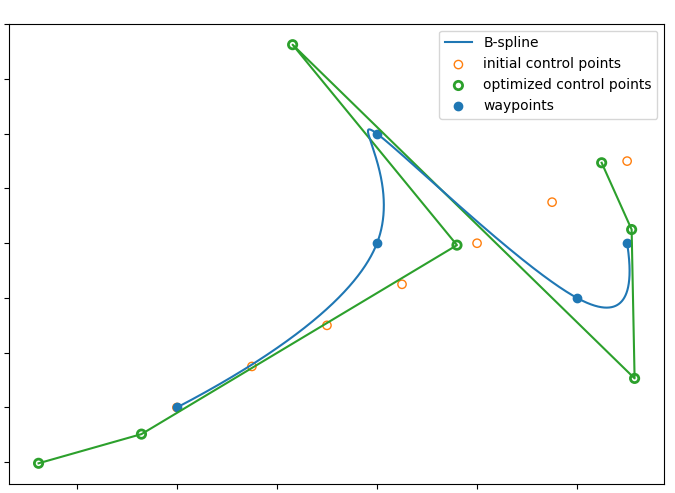
\includegraphics[scale=.5]{WaypointConstraints.png}
\end{tabular}
\caption{Set of control points constrained by waypoints}
\label{Fig:WaypointConstraints.png}
\end{figure}

    Given a set of waypoints \(\textbf{W}\), we can constrain a set of control points \(\textbf{P}\) such that the B-spline traverses through each of the waypoints at the endpoint evaluations of each knot interval of the B-spline. If we have a total of (p) waypoints, we need (p-1) defined knot point intervals.
    
    \begin{equation}
        \textbf{W} = \begin{bmatrix}
            W_0, &  W_1, & ... W_{p-1}
        \end{bmatrix}
    \end{equation}
    
    \begin{equation}
        \textbf{P} = \begin{bmatrix}
                P_0, &  P_1, & ... P_{n-1}
        \end{bmatrix}
    \end{equation}
    
   If we set 
    
    \begin{equation}
        n = k+p-1
    \end{equation}
    
We can constrain the control points as follows.

\begin{equation}
\begin{aligned}
    \forall i \in \{0 , 1 , ... w-2\} \qquad \qquad \qquad & \\
    B_i M \; L_0 & = W_i \\
    \begin{matrix} \end{matrix} \begin{bmatrix} P_i, & P_{i+1}, & ..., & P_{i+k} \end{bmatrix} M \begin{bmatrix} 0 \\ ... \\\\ 0 \\ 0 \\ 1 \end{bmatrix} & = W_i 
\end{aligned}
\end{equation}

The constraint for the last waypoint is different since we are evaluating the spline at the end of an interval instead of at the beginning.

\begin{equation}
\begin{aligned}
    B_{p-1} M \; L_f  & = W_{p-1} \\
    \begin{bmatrix} P_{p-2}, & P_{p-1}, & ..., & P_{p-2+k} \end{bmatrix} M \begin{bmatrix} 1 \\ ... \\\\ 1 \\ 1 \\ 1 \end{bmatrix} & = W_{p-1} 
\end{aligned}
\end{equation}

We can express this in shorter notation by organizing the \(M L\) vector into matrix with repeating diagonal entries.

\begin{equation}
     \textbf{M} \textbf{P}^{\intercal} = \textbf{W}^{\intercal}
\end{equation}

\begin{equation}
    \begin{bmatrix*}[l] (M \; L_0)^{\intercal} & \qquad \qquad \textbf{0} \\
    \;\; \;\; (M \; L_0)^{\intercal} & \\
    \;\; \;\; \;\; \;\; (M \; L_0)^{\intercal} & \\
    \qquad \qquad \qquad ... & \\
     & (M \; L0)^{\intercal} \;\; \;\; \;\; \;\; \\
     & \;\;\;\; (M \; L_0)^{\intercal} \;\; \;\; \\
     & \;\;\;\;\;\;\;\; (M \; L_0)^{\intercal} \\
    \;\; \textbf{0} & \;\;\;\;\;\;\;\; (M \; L_f)^{\intercal}
    \end{bmatrix*}_{\in \mathbb{R}^{p \times n}} 
    \begin{bmatrix}
        P_0^{\intercal} \\\\ P_1^\intercal \\\\ ... \\\\ P_{n-1}^\intercal
    \end{bmatrix} = 
    \begin{bmatrix} W_0^{\intercal} \\\\ W_1^{\intercal}  \\\\ ... \\\\ W_{p-1}^{\intercal} \end{bmatrix}
\end{equation}
    
\subsubsection{Variable Resolution of Knot Point intervals}

\begin{figure}[h]
\begin{tabular}{ll}
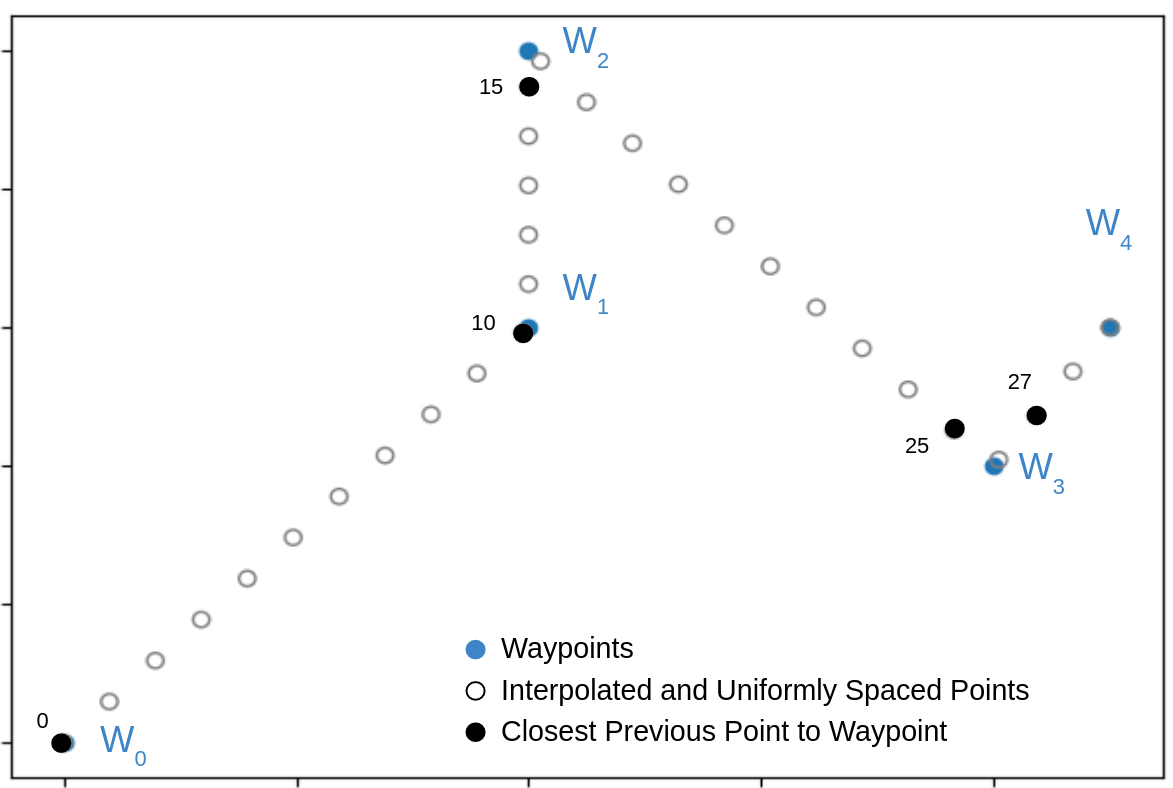
\includegraphics[scale=.35]{UniformlySpacedInterpolatedPoints.png}
\end{tabular}
\caption{Uniformly spaced points, interpolated between the desired waypoints}
\label{Fig:UniformlySpacedInterpolatedPoints}
\end{figure}

If we would like to vary the number of knot point intervals, we define (\(v\)) as the number of defined knot point intervals per B-spline. We then have the following number of control points.

\begin{equation}
    n = v + k
\end{equation}

with the requirement that the number of intervals is greater than or equal to one less of the number of waypoints.

\begin{equation}
    v \geq p-1
\end{equation}

The resolution of intervals per the length of the linear interpolation of the waypoints must also be less than the distance between each waypoint. There also cannot be consecutive repeating waypoints. This ensures that each waypoint maps to a distinct knot point interval.

\begin{equation}
    \frac{\text{Length}}{v} \leq ||W_{i+1} - W_{i}|| \quad \forall i \in \{ {0 , 1 , ..., p-2} \}
\end{equation}

We then need to determine a way of mapping each waypoint to a set of control points. This will be done by defining (n) equally spaced points, linearly interpolated between all the waypoints. See figure (\ref{Fig:UniformlySpacedInterpolatedPoints}). The point closest to each waypoint will be used to define the initial control point index of a set of control points corresponding to that waypoint. The last waypoint will always map to the (n-\textbf{k}-1) control point since (k+1) control points are needed per knot point interval. In figure (\ref{Fig:UniformlySpacedInterpolatedPoints}), this is the n-

We then generate our \(\textbf{M}\) matrix so that multiplication with the control point matrix \(\textbf{P}\) aligns the waypoints with their corresponding control points. The M matrix should look something like that shown below.

\begin{equation}
    \begin{bmatrix*}[l] (M \; L_0)^{\intercal} & \qquad \qquad \textbf{0} \\
    \;\; \;\; 0 \; 0 \; ... \; 0 & \\
    \;\; \;\; \;\; \;\; 0 \; 0 \; ... \; 0 & \\
    \qquad \qquad \qquad ... & \\
     & 0 \; 0 \; ... \; 0 \;\; \;\; \;\; \;\; \\
     & \;\;\;\; (M \; L_0)^{\intercal} \;\; \;\; \\
     & \;\;\;\;\;\;\;\; 0 \; 0 \; ... \; 0 \\
    \;\; \textbf{0} & \;\;\;\;\;\;\;\; (M \; L_f)^{\intercal}
    \end{bmatrix*}_{\in \mathbb{R}^{p \times n}} 
    \begin{bmatrix}
        P_0^{\intercal} \\\\ P_1^\intercal \\\\ ... \\\\ P_{n-1}^\intercal
    \end{bmatrix} = 
    \begin{bmatrix} W_0^{\intercal} \\\\ W_1^{\intercal}  \\\\ ... \\\\ W_{p-1}^{\intercal} \end{bmatrix}
\end{equation}

\begin{figure}[h]
\begin{tabular}{ll}
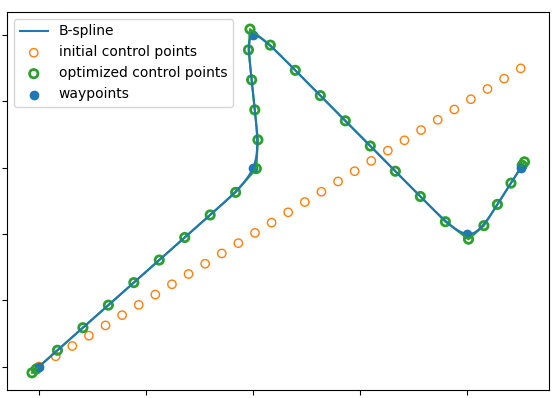
\includegraphics[scale=.6]{WaypointConstraintsVariableResolution.png}
\end{tabular}
\caption{Set of v+k control points constrained by waypoints}
\label{Fig:WaypointConstraintsVariableResolution}
\end{figure}

\subsection{Spline Derivative Constraints}

\subsubsection{Constraints on Each Spline Dimension}

Let us define the control point derivatives of a B-spline as follows.

\begin{equation}
    P_i' = \frac{P_{i+1} - P_{i}}{\alpha}
\end{equation}

\begin{equation}
   P_i''= \frac{P_{i+1}' - P_{i}'}{\alpha}
\end{equation}

or for the \(r^{th}\) derivative we have

\begin{equation}
    P_i^{(r)} = \frac{P_{i+1}^{(r-1)} - P_{i}^{(r-1)}}{\alpha}
\end{equation}

We can constrain the \(r^{th}\) derivative of a B-spline by constraining the \(r^{th}\) derivatives of the control points. In other words we can set

\begin{equation}
    b(t)^{(r)} \leq \hat{C}_{d,1}
\end{equation}

if we set the following constraints.

\begin{equation}
    \forall i \in \{0 , 1 , ... n-1\} \quad
    P_i^{(r)} \leq \hat{C}_{d,1}
\end{equation}

where \(\hat{C}_{d,1}\) is (d) dimensional array of constants for each dimension of the spline. In matrix notation we have.

\begin{equation}
\begin{aligned}
    \textbf{P}^{(r)}  & \leq \hat{C}_{d \times n-r} \\
    \begin{bmatrix}
    P_0^{(r)} & P_1^{(r)} & P_{n-r-1}^{(r)}
    \end{bmatrix}  & \leq \hat{C}_{d \times n-r} \\\\
    \frac{1}{\alpha} \begin{bmatrix}
        P_0^{(r-1)} & P_1^{(r-1)} & ... & P_{n-r}^{(r-1)}
    \end{bmatrix}
    \begin{bmatrix}
    -1 &  0 & ... & 0 & 0 \\
     1 & -1 & ... & 0 & 0 \\
     0 &  1 & ... & 0  & 0  \\
       &    & ... &   &   \\
     0  &  0 & ... & 1 & -1 \\
     0 &  0 & ... & 0 & 1 \\
    \end{bmatrix} _{\in \mathbb{R}^{n \times n-r}} & \leq 
    \begin{bmatrix}
    \hat{C}_{d,1} & \hat{C}_{d,1}  & ... & \hat{C}_{d,1} 
    \end{bmatrix}_{\in \mathbb{R}^{d \times n-r}}
\end{aligned}
\end{equation}

\subsubsection{Euclidean Distance Derivative Constraints}

\begin{figure}[h]
\begin{tabular}{ll}
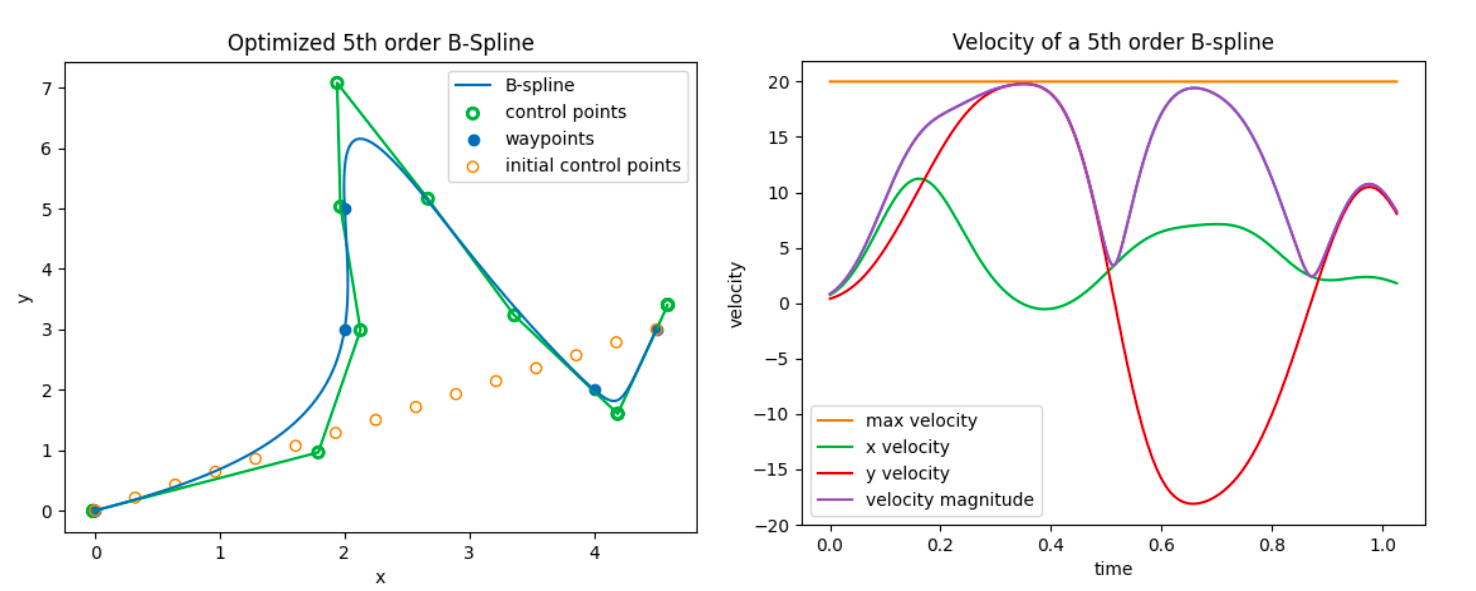
\includegraphics[scale=.28]{VelocityMagnitudeConstraint.png}
\end{tabular}
\caption{2nd order Optimized spline with waypoint and Velocity Magnitude Constraints}
\label{Fig:VelocityMagnitudeConstraint.png}
\end{figure}

Further, if we want to constrain the total magnitude the velocity, acceleration, etc.. of the spline, we can constrain the norm of the control point derivatives. For example, if we want

\begin{equation}
    ||b(t)^{(r)}||_2 \leq c \quad \forall t
\end{equation}

where \(c\) is a constant, we can set

\begin{equation}
    ||P_i^{(r)}||_2 \leq c \quad \forall i \in \{0 , 1 , ... n-1\}
\end{equation}

We can express this in matrix notation as follows.

\begin{equation}
    \begin{pmatrix}J_{1,d}(\textbf{P}^{(r)} \circ \textbf{P}^{(r)})\end{pmatrix}^{\circ \frac{1}{2}} \leq \hat{C}_{1,n-r-1} 
\end{equation}

where \(\circ\) is the hadamard product and \(^{\circ \frac{1}{2}} \) is the hadamard root and, 

\begin{equation}
J_{1,d} = \begin{bmatrix}
    1 & ... & 1
    \end{bmatrix} \in \mathbb{R}^{d}
\end{equation}

\begin{equation}
    \textbf{P}^{(r)} = \begin{bmatrix}
    P_0^{(r)} & P_1^{(r)} & ... & P_{n-r-1}^{(r)}
    \end{bmatrix}
\end{equation}

\subsubsection{Interval Endpoint Derivative Constraints}

This section describes how we can constrain the derivative of the B-spline at endpoints of each interval of the B-spline. We start by observing the equation for the matrix evaluation of a B-spline.

\begin{equation}
    b(t) = \begin{bmatrix} P_{i} & P_{i+1} & ... & P_{i+\textbf{k}}\end{bmatrix} M \begin{bmatrix} (\frac{t-t_j}{\alpha})^\textbf{k} \\ \\ ... \\ \\ (\frac{t-t_j}{\alpha})^2 \\ \\ (\frac{t-t_j}{\alpha}) \\ \\ 1 \end{bmatrix}
\end{equation}

If we take the derivative of this we get.

\begin{equation}
    b^{\prime}(t) = \begin{bmatrix} P_{i} & P_{i+1} & ... & P_{i+\textbf{k}}\end{bmatrix} M \begin{bmatrix} \frac{\textbf{k}}{\alpha} (\frac{t-t_j}{\alpha})^\textbf{k-1} \\ \\ ... \\ \\ \frac{2}{\alpha}(\frac{t-t_j}{\alpha}) \\ \\ \frac{1}{\alpha} \\ \\ 0 \end{bmatrix}
\end{equation}

We can also represent the \(r^{th}\) derivative.

\begin{equation}
    b^{(r)}(t) = \begin{bmatrix} P_{i} & P_{i+1} & ... & P_{i+\textbf{k}}\end{bmatrix} M \begin{bmatrix}
    \frac{(t-t_j)^{\textbf{k}-r} \textbf{k}!}{ \alpha^{\textbf{k}} (\textbf{k}-r)!} \\ \\ \frac{(t-t_j)^{\textbf{k}-1-r} (\textbf{k}-1)!}{ \alpha^{\textbf{k}-1} (\textbf{k}-1-r)!} \\ \\ 
    ... 
    \\ \\ 
    \frac{(t-t_j)(r+1)!}{\alpha^{r+1} 1! } 
    \\ \\ \frac{r!}{\alpha^r 0!} 
    \\ \\ \textbf{0}_{r \times 1} \end{bmatrix}
\end{equation}

where

\begin{equation}
    r \leq \textbf{k}
\end{equation}

We can now find the \(r^{th}\)derivative of the spline at the beginning of an interval.

\begin{equation}
    b^{(r)}(t_{j}) = \begin{bmatrix} P_{i} & P_{i+1} & ... & P_{i+\textbf{k}}\end{bmatrix} M \begin{bmatrix} \textbf{0}_{(\textbf{k}-r) \times 1} \\ \\ \frac{r!}{\alpha^r} \\ \\ \textbf{0}_{r \times 1} \end{bmatrix}
\end{equation}

We can also find the derivative of the spline at the end of an interval.

\begin{equation}
    b^{(r)}(t_{j+1}) = \begin{bmatrix} P_{i} & P_{i+1} & ... & P_{i+\textbf{k}}\end{bmatrix} M \begin{bmatrix}
    \frac{\textbf{k}!}{ \alpha^{r} (\textbf{k}-r)!} \\ \\ 
    \frac{ (\textbf{k}-1)!}{ \alpha^{r} (\textbf{k}-1-r)!} \\ \\ 
    ... \\ \\ 
    \frac{(r+1)!}{\alpha^{r} 1!} \\ \\ 
    \frac{r!}{\alpha^r 0!} \\ \\ 
    \textbf{0}_{r \times 1} \end{bmatrix}
\end{equation}

We can then constrain the B-spline at the interval start points to some specific value.

\begin{equation}
    \begin{bmatrix} P_{i} & P_{i+1} & ... & P_{i+\textbf{k}}\end{bmatrix} M \begin{bmatrix} \textbf{0}_{(\textbf{k}-r) \times 1} \\ \\ \frac{r!}{\alpha^r} \\ \\ \textbf{0}_{r \times 1} \end{bmatrix} = D_{i}^{(r)}
\end{equation}

The endpoint of the last interval of the B-spline is constrained as follows.

\begin{equation}
    \begin{bmatrix} P_{i} & P_{i+1} & ... & P_{i+\textbf{k}}\end{bmatrix} M \begin{bmatrix}
    \frac{\textbf{k}!}{ \alpha^{r} (\textbf{k}-r)!} \\ \\ 
    \frac{ (\textbf{k}-1)!}{ \alpha^{r} (\textbf{k}-1-r)!} \\ \\ 
    ... \\ \\ 
    \frac{(r+1)!}{\alpha^{r} 1!} \\ \\ 
    \frac{r!}{\alpha^r 0!} \\ \\ 
    \textbf{0}_{r \times 1} \end{bmatrix} = D_{i+1}^{(r)}
\end{equation}

Given a set of \(\textbf{D}^{(r)}\) derivative values, we can constrain the specific interval endpoints to those values. Like in section \ref{Minimum Number of Knot Point Intervals}, we set up a matrix with repeating diagonal entries.

\begin{equation}
    \textbf{M}  \textbf{P}^{\intercal} = \textbf{D}^{(r) \intercal}
\end{equation}

\begin{equation} \label{Point_Derivative_Constraints}
    \begin{bmatrix*}[l] (M \; L_0^{(r)})^{\intercal} & \qquad \qquad \textbf{0} \\
    \;\; \;\; (M \; L_0^{(r)})^{\intercal} & \\
    \;\; \;\; \;\; \;\; (M \; L_0^{(r)})^{\intercal} & \\
    \qquad \qquad \qquad ... & \\
     & (M \; L_0^{(r)})^{\intercal} \;\; \;\; \;\; \;\; \\
     & \;\;\;\; (M \; L_0^{(r)})^{\intercal} \;\; \;\; \\
     & \;\;\;\;\;\;\;\; (M \; L_0^{(r)})^{\intercal} \\
    \;\; \textbf{0} & \;\;\;\;\;\;\;\; (M \; L_f^{(r)})^{\intercal}
    \end{bmatrix*}_{\in \mathbb{R}^{p \times n}} 
    \begin{bmatrix}
        P_0^{\intercal} \\\\ P_1^\intercal \\\\ ... \\\\ P_{n-1}^\intercal
    \end{bmatrix} = 
    \begin{bmatrix} D_0^{(r)\intercal} \\\\ D_1^{(r)\intercal}  \\\\ ... \\\\ D_{p-1}^{(r)\intercal} \end{bmatrix}
\end{equation}

where 

\begin{equation}
L_0^{(r)} = \begin{bmatrix} \textbf{0}_{(\textbf{k}-r) \times 1} \\ \\ \frac{r!}{\alpha^r} \\ \\ \textbf{0}_{r \times 1} \end{bmatrix}
\end{equation}

\begin{equation}
L_f^{(r)} = \begin{bmatrix}
    \frac{\textbf{k}!}{ \alpha^{r} (\textbf{k}-r)!} \\ \\ 
    \frac{ (\textbf{k}-1)!}{ \alpha^{r} (\textbf{k}-1-r)!} \\ \\ 
    ... \\ \\ 
    \frac{(r+1)!}{\alpha^{r} 1!} \\ \\ 
    \frac{r!}{\alpha^r 0!} \\ \\ 
    \textbf{0}_{r \times 1} \end{bmatrix}
\end{equation}

If we would like to constrain only the derivatives at the first and last waypoint, the matrix equation is setup as follows.

\begin{equation}
    \begin{bmatrix*}[l] (M \; L_0^{(r)})^{\intercal} & \qquad \qquad \textbf{0} \\
    \;\; \textbf{0} & \;\;\;\;\;\;\;\; (M \; L_f^{(r)})^{\intercal}
    \end{bmatrix*}_{\in \mathbb{R}^{2 \times n}} 
    \begin{bmatrix}
        P_0^{\intercal} \\\\ P_1^\intercal \\\\ ... \\\\ P_{n-1}^\intercal
    \end{bmatrix} = 
    \begin{bmatrix} D_0^{(r)\intercal} \\\\ D_{p-1}^{(r)\intercal} \end{bmatrix}
\end{equation}

\subsubsection{Interval Endpoint Euclidean Distance Derivative Constraints}

If we would like to constrain the total magnitude of the velocity, acceleration, etc.. at the start point of a knot interval we can constrain the control points as follows.

\begin{equation}
   || \begin{bmatrix} P_{i} & P_{i+1} & ... & P_{i+\textbf{k}}\end{bmatrix} M L_0^{(r)} ||_2 = C_i
\end{equation}

We can constrain the endpoint of a knot interval just the same.

\begin{equation}
   || \begin{bmatrix} P_{i} & P_{i+1} & ... & P_{i+\textbf{k}}\end{bmatrix} M L_f^{(r)} ||_2 = C_{i+1}
\end{equation}

We can represent these constraints for all the knot interval start and endpoints as follows.

\begin{equation} \label{Derivative Magnitude Constraint}
\begin{aligned}
( \textbf{M} \textbf{P}^{\intercal} \circ \textbf{M} \textbf{P}^{\intercal} J_{d,1})^{\circ \frac{1}{2}} \begin{bmatrix}
1 \\ 1 \\ ... \\ 1
\end{bmatrix}_{\in \mathbb{R}^{d}} & = C^{\intercal} \\ \\
    \begin{pmatrix} \begin{pmatrix} \begin{bmatrix*}[l] (M \; L_0^{(r)})^{\intercal} & \qquad \qquad \textbf{0} \\
    \;\; \;\; (M \; L_0^{(r)})^{\intercal} & \\
    \;\; \;\; \;\; \;\; (M \; L_0^{(r)})^{\intercal} & \\
    \qquad \qquad \qquad ... & \\
     & (M \; L_0^{(r)})^{\intercal} \;\; \;\; \;\; \;\; \\
     & \;\;\;\; (M \; L_0^{(r)})^{\intercal} \;\; \;\; \\
     & \;\;\;\;\;\;\;\; (M \; L_0^{(r)})^{\intercal} \\
    \;\; \textbf{0} & \;\;\;\;\;\;\;\; (M \; L_f^{(r)})^{\intercal}
    \end{bmatrix*}_{\in \mathbb{R}^{p \times n}}
    \begin{bmatrix}
        P_0^{\intercal} \\\\ P_1^\intercal \\\\ ... \\\\ P_{n-1}^\intercal
    \end{bmatrix}\end{pmatrix}^{\circ 2} \begin{bmatrix} 1 \\ 1 \\ ... \\ 1 \end{bmatrix}_{\in \mathbb{R}^{d}} \end{pmatrix}^{\circ \frac{1}{2}} & = \begin{bmatrix}
    C_1 \\ C_2 \\ .. \\ C_{n-1}
    \end{bmatrix}
\end{aligned}
\end{equation}


\subsubsection{Directional Constraints}

To constrain the direction of the spline at the endpoint of an interval, we simply constrain the angles defining the direction gradient vector of the b-spline. The velocity at the beginning of an interval is shown below.

\begin{equation}
    v(t_{j}) = \begin{bmatrix} P_{i} & P_{i+1} & ... & P_{i+\textbf{k}}\end{bmatrix} M L_0^{'}
\end{equation}

Below is the velocity of the spline at the end of an interval.

\begin{equation}
    v(t_{j+1}) = \begin{bmatrix} P_{i} & P_{i+1} & ... & P_{i+\textbf{k}}\end{bmatrix} M L_f^{'}
\end{equation}

where 

\begin{equation}
    L_0^{'} = \begin{bmatrix} \textbf{0}_{(\textbf{k}-1) \times 1} \\ \\ \frac{1}{\alpha} \\ \\ 0 \end{bmatrix} , \qquad L_f^{'} = \begin{bmatrix}
    \frac{\textbf{k}}{ \alpha} \\ \\ 
    \frac{\textbf{k-1}}{ \alpha} \\ \\ 
    ... \\ \\ 
    \frac{2}{\alpha} \\ \\ 
    \frac{1}{\alpha} \\ \\ 
    0\end{bmatrix}
\end{equation}

where

\begin{equation}
    v(t_j) = \begin{bmatrix} \nu_x(t_j) \\ \nu_y(t_j) \\ \nu_z(t_j) \end{bmatrix}
\end{equation}

\begin{figure}[h]
\begin{tabular}{ll}
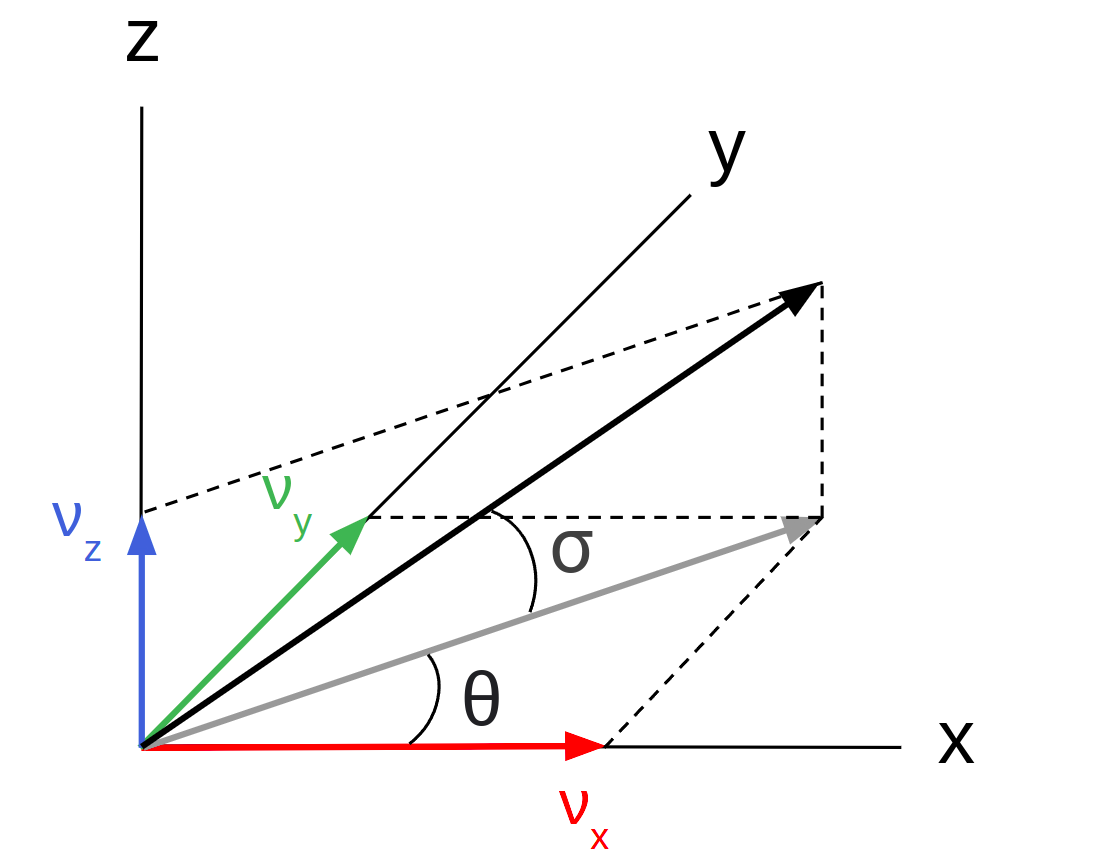
\includegraphics[scale=.3]{directions.png}
\end{tabular}
\caption{Defining the direction of the spline at a point}
\label{Fig:directions.png}
\end{figure}

The direction is constrained as follows.

\begin{equation}
    \theta_j = \tan^{-1} \Big( \frac{\nu_y(t_j)}{\nu_x(t_j)}\Big)
\end{equation}

\begin{equation}
    \sigma_j = \tan^{-1} \Big(\frac{\nu_z(t_j)}{\nu_x(t_j)\cos\theta + \nu_y(t_j) \sin\theta}  \Big)
\end{equation}

\subsection{Curve Shape Constraints}

\subsubsection{Curvature}

The curvature of a function at a specific point is defined by the circle that best approximates the shape of the curve at that point. It is formally defined by the inverse radius of the circle. See figure \ref{Fig:Curvature}. 

\begin{figure}[h]
\begin{center}
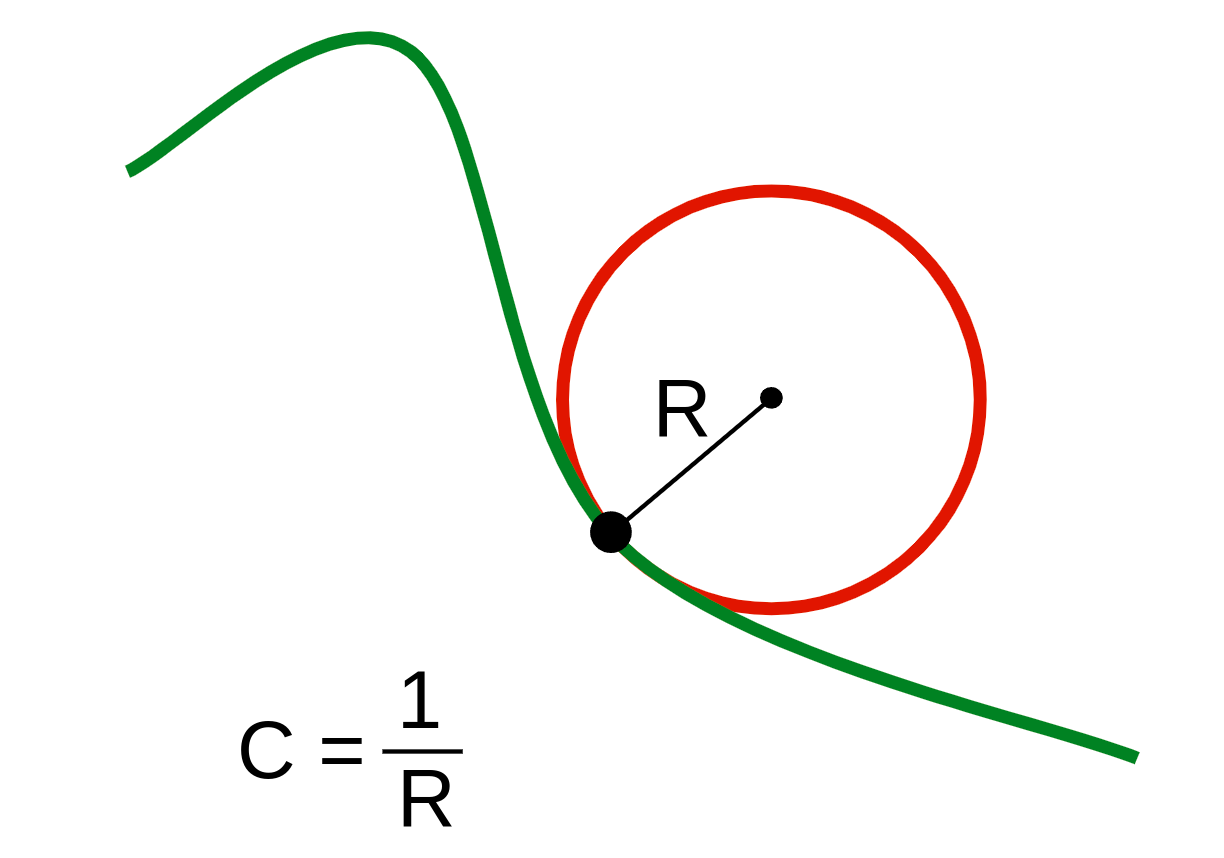
\includegraphics[scale=.13]{Curvature.png}
\end{center}
\caption{Curvature defined by the oscillating circle}
\label{Fig:Curvature}
\end{figure}

Curvature of a spline can be evaluated by the following equation.

\begin{equation} \label{eq:Curvature}
    C(t) = \frac{||b(t)' \times b(t)''||}{||b(t)'||^3} = \frac{||\nu \times a||}{||\nu||^3}
\end{equation}

We can directly constrain the curvature for the bicycle model, or simplified car models that do not consider slip.

\subsubsection{Angular Rate}

Here we refer to the angular rate of the tangent vector of the path as it progresses along the trajectory. Angular rate is defined by the tangent velocity and radius of the oscillating circle that the path is approximating. See figure \ref{Fig:AngularRate.png}.

\begin{figure}[h]
\centering
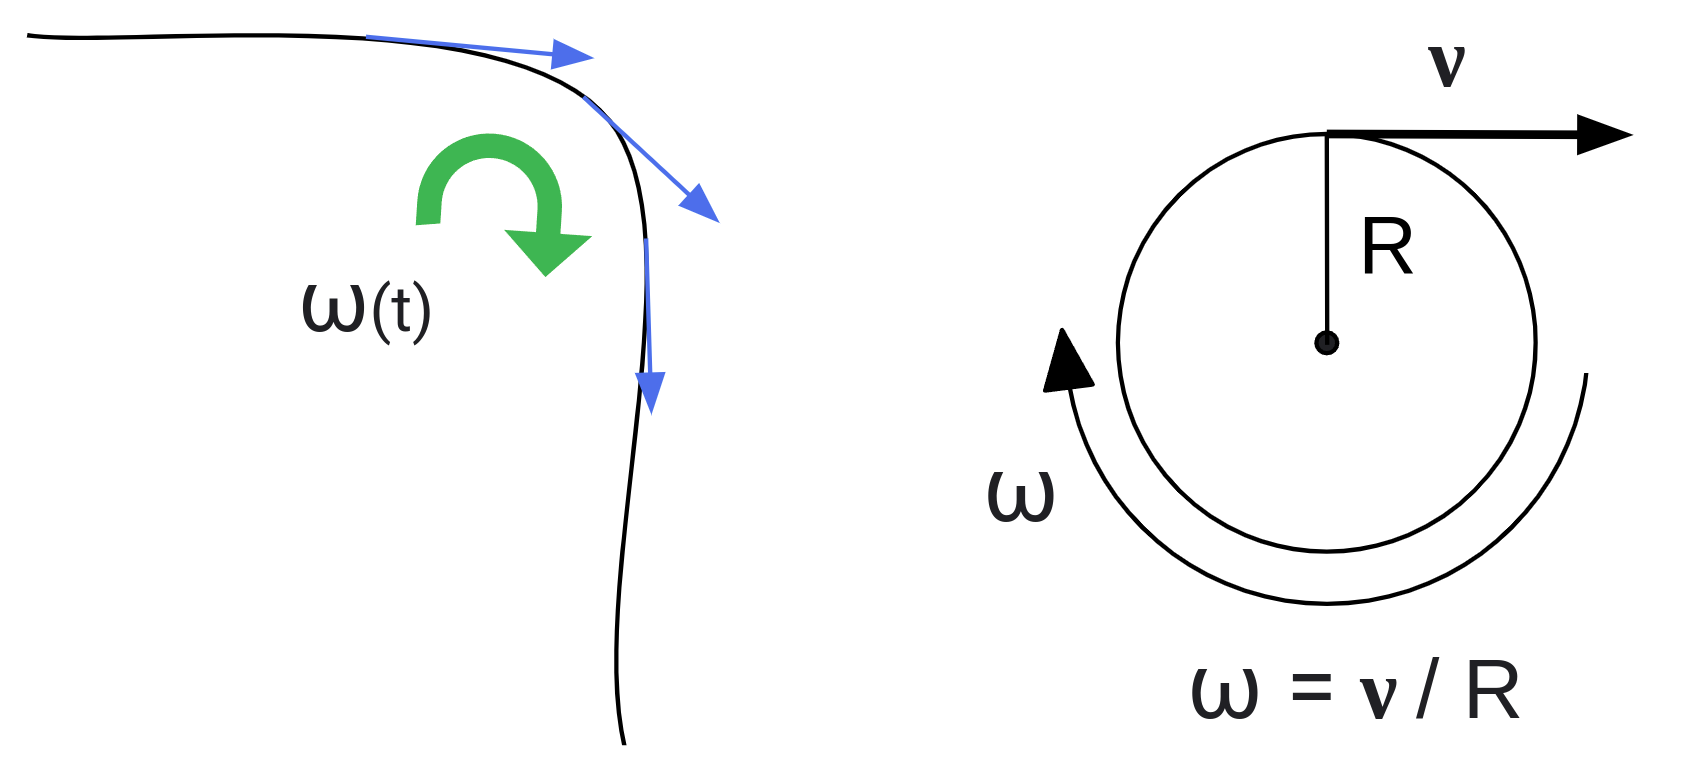
\includegraphics[scale=.12]{AngularRate.png}
\caption{Angular Rate along a path}
\label{Fig:AngularRate.png}
\end{figure}

\begin{equation}
    \omega = \frac{\nu}{R} = \nu C
\end{equation}

Using the curvature equation we get the following equation for the angular rate.
\begin{equation}
    \omega(t) = \frac{||b(t)' \times b(t)''||}{||b(t)'||^2} = \frac{||\nu \times a||}{||\nu||^2}
\end{equation}

For vehicle models like the unicycle model, or a quadrotor model, we can directly constrain the angular rate.

\subsubsection{Centripetal Acceleration}

The centripetal acceleration is the portion of acceleration that is perpendicular to the velocity vector. See figure \ref{Centripetal_Acceleration}.

\begin{figure}[h]
\centering
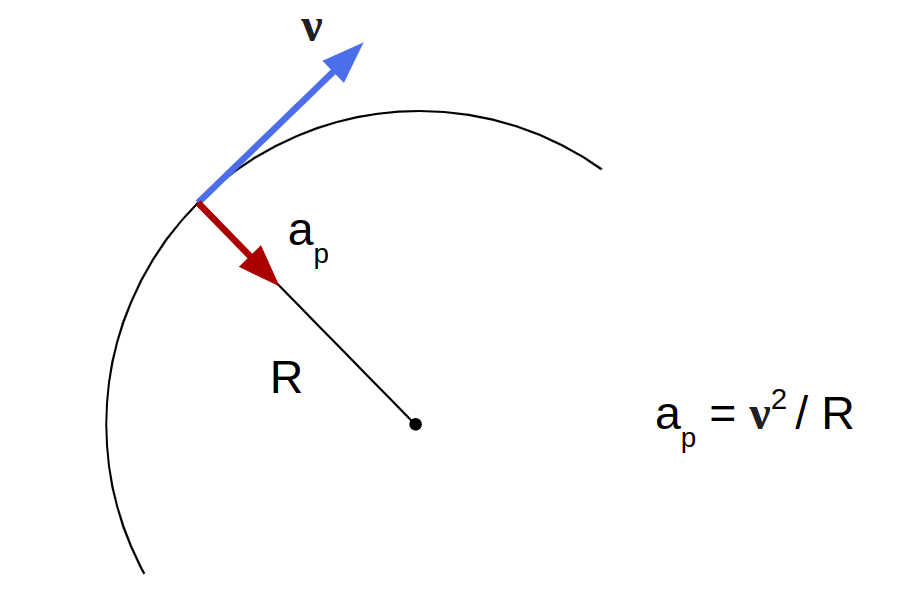
\includegraphics[scale=.22]{CentripetalAcceleration.png}
\caption{Centripetal Acceleration}
\label{Centripetal_Acceleration}
\end{figure}

\begin{equation} \label{eq:Centripetal Physics}
    a_p = \frac{\nu^2}{R} = \nu^2 C
\end{equation}

We can derive the equation for centripetal acceleration with equations (\ref{eq:Curvature}) and (\ref{eq:Centripetal Physics}).

\begin{equation}
    a_p = \frac{||b(t)' \times b(t)''||}{||b(t)'||} = \frac{||\nu \times a||}{||\nu||}
\end{equation}

\subsection{Bezier Curves}


\subsection{Obstacle Avoidance Constraints}

\section{Optimizing Trajectories using B-Splines}

\subsection{Minimizing Snap}

Snap is the fourth derivative of the position. This is minimized because the input variables to some UAV's are algebraically related to snap. We start by deriving the equation for snap.


\begin{equation}
    b^{''''}(t) = \begin{bmatrix} P_{i} & P_{i+1} & ... & P_{i+\textbf{k}}\end{bmatrix} M \begin{bmatrix}
    \frac{120(t-t_j)}{ \alpha^{5}} \\ \\ 
    \frac{24}{\alpha^{4}} \\ \\ 
    ... \\ \\ 
    \frac{(r+1)!}{\alpha^{r} 1!} \\ \\ 
    \frac{r!}{\alpha^r 0!} \\ \\ 
    \textbf{0}_{r \times 1} \end{bmatrix}
\end{equation}


\section{Appendix}

The hadamard product is the element wise product or entrywise product of two matrices.

\begin{equation}
    \begin{bmatrix}
    a_{11} & a_{12} & a_{13} \\
    a_{21} & a_{22} & a_{23} \\
    a_{31} & a_{32} & a_{33}
    \end{bmatrix} \circ
    \begin{bmatrix}
    b_{11} & b_{12} & b_{13} \\
    b_{21} & b_{22} & b_{23} \\
    b_{31} & b_{32} & b_{33}
    \end{bmatrix} = 
    \begin{bmatrix}
    a_{11}b_{11} & a_{12}b_{12} & a_{13}b_{13} \\
    a_{21}b_{21} & a_{22}b_{22} & a_{23}b_{23} \\
    a_{31}b_{31} & a_{32}b_{32} & a_{33}b_{33}
    \end{bmatrix}
\end{equation}

\end{document}


